% Options for packages loaded elsewhere
% Options for packages loaded elsewhere
\PassOptionsToPackage{unicode}{hyperref}
\PassOptionsToPackage{hyphens}{url}
\PassOptionsToPackage{dvipsnames,svgnames,x11names}{xcolor}
%
\documentclass[
  letterpaper,
  DIV=11,
  numbers=noendperiod]{scrartcl}
\usepackage{xcolor}
\usepackage{amsmath,amssymb}
\setcounter{secnumdepth}{-\maxdimen} % remove section numbering
\usepackage{iftex}
\ifPDFTeX
  \usepackage[T1]{fontenc}
  \usepackage[utf8]{inputenc}
  \usepackage{textcomp} % provide euro and other symbols
\else % if luatex or xetex
  \usepackage{unicode-math} % this also loads fontspec
  \defaultfontfeatures{Scale=MatchLowercase}
  \defaultfontfeatures[\rmfamily]{Ligatures=TeX,Scale=1}
\fi
\usepackage{lmodern}
\ifPDFTeX\else
  % xetex/luatex font selection
\fi
% Use upquote if available, for straight quotes in verbatim environments
\IfFileExists{upquote.sty}{\usepackage{upquote}}{}
\IfFileExists{microtype.sty}{% use microtype if available
  \usepackage[]{microtype}
  \UseMicrotypeSet[protrusion]{basicmath} % disable protrusion for tt fonts
}{}
\makeatletter
\@ifundefined{KOMAClassName}{% if non-KOMA class
  \IfFileExists{parskip.sty}{%
    \usepackage{parskip}
  }{% else
    \setlength{\parindent}{0pt}
    \setlength{\parskip}{6pt plus 2pt minus 1pt}}
}{% if KOMA class
  \KOMAoptions{parskip=half}}
\makeatother
% Make \paragraph and \subparagraph free-standing
\makeatletter
\ifx\paragraph\undefined\else
  \let\oldparagraph\paragraph
  \renewcommand{\paragraph}{
    \@ifstar
      \xxxParagraphStar
      \xxxParagraphNoStar
  }
  \newcommand{\xxxParagraphStar}[1]{\oldparagraph*{#1}\mbox{}}
  \newcommand{\xxxParagraphNoStar}[1]{\oldparagraph{#1}\mbox{}}
\fi
\ifx\subparagraph\undefined\else
  \let\oldsubparagraph\subparagraph
  \renewcommand{\subparagraph}{
    \@ifstar
      \xxxSubParagraphStar
      \xxxSubParagraphNoStar
  }
  \newcommand{\xxxSubParagraphStar}[1]{\oldsubparagraph*{#1}\mbox{}}
  \newcommand{\xxxSubParagraphNoStar}[1]{\oldsubparagraph{#1}\mbox{}}
\fi
\makeatother


\usepackage{longtable,booktabs,array}
\newcounter{none} % for unnumbered tables
\usepackage{calc} % for calculating minipage widths
% Correct order of tables after \paragraph or \subparagraph
\usepackage{etoolbox}
\makeatletter
\patchcmd\longtable{\par}{\if@noskipsec\mbox{}\fi\par}{}{}
\makeatother
% Allow footnotes in longtable head/foot
\IfFileExists{footnotehyper.sty}{\usepackage{footnotehyper}}{\usepackage{footnote}}
\makesavenoteenv{longtable}
\usepackage{graphicx}
\makeatletter
\newsavebox\pandoc@box
\newcommand*\pandocbounded[1]{% scales image to fit in text height/width
  \sbox\pandoc@box{#1}%
  \Gscale@div\@tempa{\textheight}{\dimexpr\ht\pandoc@box+\dp\pandoc@box\relax}%
  \Gscale@div\@tempb{\linewidth}{\wd\pandoc@box}%
  \ifdim\@tempb\p@<\@tempa\p@\let\@tempa\@tempb\fi% select the smaller of both
  \ifdim\@tempa\p@<\p@\scalebox{\@tempa}{\usebox\pandoc@box}%
  \else\usebox{\pandoc@box}%
  \fi%
}
% Set default figure placement to htbp
\def\fps@figure{htbp}
\makeatother


% definitions for citeproc citations
\NewDocumentCommand\citeproctext{}{}
\NewDocumentCommand\citeproc{mm}{%
  \begingroup\def\citeproctext{#2}\cite{#1}\endgroup}
\makeatletter
 % allow citations to break across lines
 \let\@cite@ofmt\@firstofone
 % avoid brackets around text for \cite:
 \def\@biblabel#1{}
 \def\@cite#1#2{{#1\if@tempswa , #2\fi}}
\makeatother
\newlength{\cslhangindent}
\setlength{\cslhangindent}{1.5em}
\newlength{\csllabelwidth}
\setlength{\csllabelwidth}{3em}
\newenvironment{CSLReferences}[2] % #1 hanging-indent, #2 entry-spacing
 {\begin{list}{}{%
  \setlength{\itemindent}{0pt}
  \setlength{\leftmargin}{0pt}
  \setlength{\parsep}{0pt}
  % turn on hanging indent if param 1 is 1
  \ifodd #1
   \setlength{\leftmargin}{\cslhangindent}
   \setlength{\itemindent}{-1\cslhangindent}
  \fi
  % set entry spacing
  \setlength{\itemsep}{#2\baselineskip}}}
 {\end{list}}
\usepackage{calc}
\newcommand{\CSLBlock}[1]{\hfill\break\parbox[t]{\linewidth}{\strut\ignorespaces#1\strut}}
\newcommand{\CSLLeftMargin}[1]{\parbox[t]{\csllabelwidth}{\strut#1\strut}}
\newcommand{\CSLRightInline}[1]{\parbox[t]{\linewidth - \csllabelwidth}{\strut#1\strut}}
\newcommand{\CSLIndent}[1]{\hspace{\cslhangindent}#1}



\setlength{\emergencystretch}{3em} % prevent overfull lines

\providecommand{\tightlist}{%
  \setlength{\itemsep}{0pt}\setlength{\parskip}{0pt}}



 


\usepackage{float}
\usepackage{tabularray}
\usepackage[normalem]{ulem}
\usepackage{graphicx}
\usepackage{rotating}
\UseTblrLibrary{siunitx}
\NewTableCommand{\tinytableDefineColor}[3]{\definecolor{#1}{#2}{#3}}
\newcommand{\tinytableTabularrayUnderline}[1]{\underline{#1}}
\newcommand{\tinytableTabularrayStrikeout}[1]{\sout{#1}}
\KOMAoption{captions}{tableheading}
\makeatletter
\@ifpackageloaded{caption}{}{\usepackage{caption}}
\AtBeginDocument{%
\ifdefined\contentsname
  \renewcommand*\contentsname{Table of contents}
\else
  \newcommand\contentsname{Table of contents}
\fi
\ifdefined\listfigurename
  \renewcommand*\listfigurename{List of Figures}
\else
  \newcommand\listfigurename{List of Figures}
\fi
\ifdefined\listtablename
  \renewcommand*\listtablename{List of Tables}
\else
  \newcommand\listtablename{List of Tables}
\fi
\ifdefined\figurename
  \renewcommand*\figurename{Figure}
\else
  \newcommand\figurename{Figure}
\fi
\ifdefined\tablename
  \renewcommand*\tablename{Table}
\else
  \newcommand\tablename{Table}
\fi
}
\@ifpackageloaded{float}{}{\usepackage{float}}
\floatstyle{ruled}
\@ifundefined{c@chapter}{\newfloat{codelisting}{h}{lop}}{\newfloat{codelisting}{h}{lop}[chapter]}
\floatname{codelisting}{Listing}
\newcommand*\listoflistings{\listof{codelisting}{List of Listings}}
\makeatother
\makeatletter
\makeatother
\makeatletter
\@ifpackageloaded{caption}{}{\usepackage{caption}}
\@ifpackageloaded{subcaption}{}{\usepackage{subcaption}}
\makeatother
\usepackage{bookmark}
\IfFileExists{xurl.sty}{\usepackage{xurl}}{} % add URL line breaks if available
\urlstyle{same}
\hypersetup{
  pdftitle={How does familiarity impact the computational processes that support face recognition?},
  pdfauthor={Raphaël Fournier; Paul Downing; Richard Ramsey},
  pdfkeywords={face perception, memory, familiarity, person
knowledge, decision models, evidence accumulation modelling},
  colorlinks=true,
  linkcolor={blue},
  filecolor={Maroon},
  citecolor={Blue},
  urlcolor={Blue},
  pdfcreator={LaTeX via pandoc}}


\title{How does familiarity impact the computational processes that
support face recognition?}
\author{Raphaël Fournier \and Paul Downing \and Richard Ramsey}
\date{2026-08-10}
\begin{document}
\maketitle
\begin{abstract}
Recognising a familiar face is a fundamental social cognitive ability,
yet the computational mechanisms that underlie this capacity remain
poorly understood. Prior research has established that familiarity
affects face recognition performance, but has relied primarily on
manifest measures --- accuracy and response time --- that cannot
distinguish between qualitatively different sources of performance
change. Here, we used evidence accumulation modelling across a series of
experiments to ask not merely whether familiarity affects face
recognition, but how --- specifically, which latent computational
processes are modulated. Experiments 1 and 2 examined visual familiarity
(briefly learned faces versus novel faces) and Experiments 3, 4 and 5
examined person knowledge (famous versus novel faces). Fitting linear
ballistic accumulator models to recognition data revealed a consistent
computational signature across experiments: novel faces produced
substantially higher drift rates than familiar faces, accompanied by a
smaller but reliable increase in response caution. The dominance of the
drift rate effect localises familiarity's primary influence to the
quality of evidence accumulation --- how cleanly the perceptual system
extracts decision-relevant information --- rather than to response bias.
We interpret thes findings as reflecting a novelty pop-out effect
combined with unstable memory traces for familiar faces. These findings
demonstrate that computational modelling reveals dissociable mechanisms
underlying face recognition that are invisible to manifest measures
alone, and provide a foundation for understanding how familiarity shapes
the decision processes that support social perception.
\end{abstract}


\newpage{}

\section{Introduction}\label{introduction}

The ability to quickly and accurately recognise a familiar face is an
important aspect of everyday life, as it guides social behaviour. The
way that one might interact with a family member or friend is different
to a stranger. Moreover, for familiar individuals, we not only know what
they look like, but we also have access to person knowledge, such as
their traits, attitudes, name and professional status. To date, most
prior face recognition research has used manifest (observed) measures
(i.e., response times and accuracy) to assess one's ability to recognise
faces. As such, less is known about the latent computational processes
that support face recognition (Phillips \& White, 2025). In the current
project, we investigated how different types of familiarity, including
visual feature familiarity and stored person knowledge, affected the
latent processes that can be estimated by evidence accumulation models
(EAMs; Ratcliff \& Rouder (1998)). This computational approach has
provided new insights on the dynamics of the decision process supporting
face recognition.

The structure of mental processes that support face recognition has been
a topic of investigation over the last 50 years (R. A. Johnston \&
Edmonds, 2009; Natu \& O'Toole, 2011). One influential cognitive model
of face recognition proposed a division between structural encoding of
facial features, and more elaborate processes associated with identity
recognition and person information (Bruce \& Young, 1986). Subsequent
neuroscience research in humans and monkeys has enriched this model by
relating different cognitive processes to different brain circuits
Gobbini \& Haxby (2006). The resulting model is a distributed neural
network that incorporates two distinct systems: a core system and an
extended system. The core system is dedicated to structural coding of
facial features. In contrast, the extended system is involved in more
elaborate processes, such as those related to person knowledge (Duchaine
\& Yovel, 2015; Gobbini \& Haxby, 2007; Haxby et al., 2000; Ishai, 2008;
Kanwisher \& Barton, 2011). By mediating the retrieval of
identity-specific information from memory, the extended system is able
to support the recognition of faces for which prior person knowledge
information has been stored (Ida Gobbini et al., 2004; Leibenluft et
al., 2004).

Given the importance of knowing who it is you are interacting with, the
study of familiarity has been a key aspect of the face perception
research (Young \& Burton, 2018). Largely using manifest measures, such
as response time and accuracy, research consistently shows that familiar
faces, especially those imbued with person knowledge, facilitate a range
of face recognition processes compared to previously unseen individuals
or visually familiar faces (Ramon \& Gobbini, 2018; Young \& Burton,
2018). It has been argued that person knowledge involves a qualitatively
different and deeper level of processing than visual familiarity
(Schwartz \& Yovel, 2019), which facilitates the accurate discrimination
of familiar from unfamiliar faces (Akan \& Benjamin, 2023, 2023; Bird et
al., 2011; Klatzky \& Forrest, 1984; Schwaninger et al., 2002; Schwartz
\& Yovel, 2016).

Although manifest (observed) measures of performance have formed the
bedrock of research findings on face perception, there have been many
calls in recent years to embrace more computational approaches in social
and cognitive neuroscience research (Charpentier \& O'Doherty, 2018;
Cheong et al., 2017; Forstmann \& Turner, 2024; Hackel \& Amodio, 2018;
Lockwood \& Klein-Flügge, 2021; Parker \& Ramsey, 2024; Phillips \&
White, 2025). One benefit of adopting computational approaches is that
relationships between parts of a system can be more explicitly specified
(Hintzman, 1991; Yarkoni, 2022), which aids the development of theory
(Muthukrishna \& Henrich, 2019; Oberauer \& Lewandowsky, 2019; Proulx \&
Morey, 2021). A second benefit is that latent (unobserved) parameters
can be estimated, which can give rise to different interpretations of
the cognitive processes involved in task performance (Ratcliff et al.,
2001). And at present, there is almost no understanding of the
computational processes that support face recognition processes when
familiarity is based on visual exposure compared to stored person
knowledge (Phillips \& White, 2025).

Evidence accumulation models (EAM) are one approach to investigate the
computational processes that are involved in speeded decision tasks (for
a review, see Ratcliff et al. (2016)). While a variety of different
evidence accumulation models exists, they all share a similar set of
assumptions: that evidence for each response option accumulates at
different rates until one response option crosses a threshold and a
response is triggered (see Figure~\ref{fig-LBA} for an example of the
linear ballistic accumulator (LBA) model; Brown \& Heathcote (2008)).
These models work by translating the distribution of response times for
correct and incorrect responses into estimates of latent variables
assumed to underlie the decision-making process Table~\ref{tbl-lba}.
These latent variables can then be mapped onto psychological constructs
(Myers et al., 2022). For example, drift rate is the rate at which
evidence in favor of a decision accumulates over time, reflecting the
signal-to-noise ratio provided by the stimulus. Threshold represents the
amount of accumulated evidence needed to trigger the decision,
reflecting the response caution towards a specific response. The
starting point is the amount of evidence towards a response before the
accumulation of evidence begins, reflecting the \emph{a priori} bias
towards a response. Finally, the non-decision time is an estimation of
the time taken to complete processes that are not involved in the
decision time, such as stimulus encoding and motor responses.

\begin{figure}

\centering{

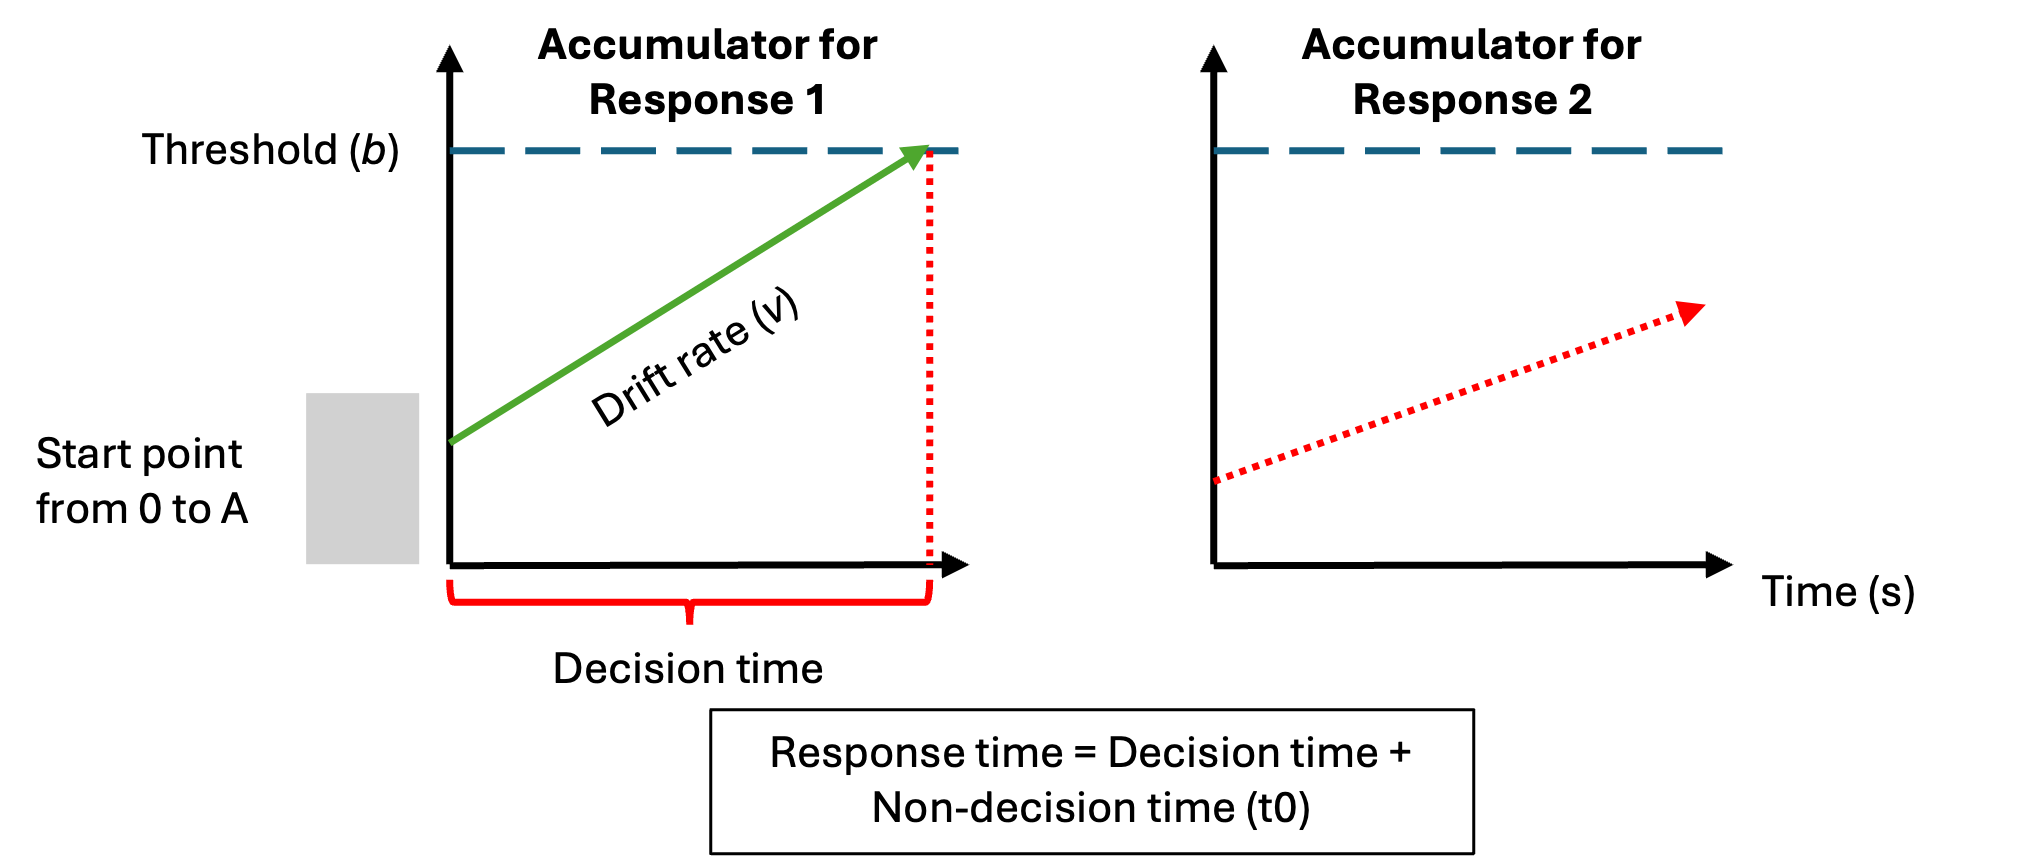
\includegraphics[width=0.9\linewidth,height=\textheight,keepaspectratio]{figures/LBA_schematique.png}

}

\caption{\label{fig-LBA}Schematic of the linear ballistic accumulator
(LBA) model}

\end{figure}%

\emph{This diagram represents the accumulation process one trial of a
perceptual decision task for the linear ballistic accumulator (LBA).
Participants are required to chose between two options (Response 1 and
Response 2). In a LBA model, there is a separated accumulation of
evidence (v) for each response option. In this example, the correct
response is Response 1. The accumulator on the left is the accumulator
for the correct response (Response 1), and the green line in represents
the rate at which the evidence accumulates in favor of that response
option. The accumulator on the right is the accumulator for the
incorrect response (Response 2), and the dash red line represents the
rate at which the evidence accumulates in favor of this response option.
Once the accumulated evidence crosses the threshold (b) of a response
option, the corresponding response is chosen (in this case Response 1).}

\begin{table}

\caption{\label{tbl-lba}Parameters in the linear ballistic accumulator
model}

\centering{

\centering
\begin{tblr}[         %% tabularray outer open
]                     %% tabularray outer close
{                     %% tabularray inner open
colspec={Q[]Q[]Q[]},
hline{2}={1-3}{solid, black, 0.05em},
hline{1}={1-3}{solid, black, 0.08em},
hline{6}={1-3}{solid, black, 0.08em},
}                     %% tabularray inner close
Parameter & Label & Construct \\
Start point & A & response bias \\
Drift rate & v & signal-to-noise ratio \\
Threshold & b & response caution \\
Non-decision time & t#sub[0] & stimulus encoding and motor response \\
\end{tblr}

}

\end{table}%

In the present study, we used evidence accumulation modelling to ask new
questions regarding the computational processes that support the
recognition of familiar versus unfamiliar individuals. More
specifically, we address how different types of familiarity (visual
feature familiarity versus visual feature familiarity plus person
knowledge) impact the threshold (response caution) and drift rate
(signal-to-noise ratio) parameters. Based on prior work in experimental
psychology (Parker \& Ramsey, 2024; Ratcliff et al., 2016), we chose to
primarily focus on threshold and drift rate as our primary parameters of
interest because we could easily and intuitively see how performance
advantages could emerge based on familiarity. For instance, based on
conventional use of EAMs (Myers et al., 2022), increases in
signal-to-noise ratio and/or reductions in response caution could be
interpreted as the task setting becoming easier.

We, therefore, hypothesised that either drift rate and/or threshold
would be affected by the face familiarity manipulation. However, given
the general lack of prior evidence accumulation modelling in face
recognition research, we were unsure \emph{a priori} of the direction of
the effects. For instance, we considered it plausible that novel
compared to familiar stimuli could provide a benefit in some instances,
by virtue of a pop-out or novelty detector (Glanzer \& Adams, 1985;
Kormi-Nouri et al., 2005; Schomaker \& Meeter, 2012; Tulving \& Kroll,
1995). Likewise, we also considered it plausible that familiar compared
to novel stimuli could providing a benefit based on the many advantages
reported for recognising personally familiar or famous individuals
(Ramon \& Gobbini, 2018; Young \& Burton, 2018). Nonetheless, across a
series of experiments, we used manipulations of familiarity that either
only targeted the operation of core system only or the core and extended
system of face perception (Table~\ref{tbl-exp}), so that we could
further understand the computational processes that underpin different
types of familiar face recognition.

\begin{table}

\caption{\label{tbl-exp}An overview of the experimental work}

\centering{

\centering
\begin{tblr}[         %% tabularray outer open
]                     %% tabularray outer close
{                     %% tabularray inner open
colspec={Q[]Q[]Q[]Q[]Q[]},
hline{2}={1-5}{solid, black, 0.05em},
hline{1}={1-5}{solid, black, 0.08em},
hline{7}={1-5}{solid, black, 0.08em},
}                     %% tabularray inner close
Exp & Setting & Familiarity type & Face comparision & Face system \\
1 & laboratory & visual & visual exposure vs unknown & core \\
2 & online & visual & visual exposure vs unknown & core \\
3 & laboratory & visual & person knowledge & famous vs unknown & core & extended \\
4 & online & visual & person knowledge & famous vs unknown & core & extended \\
5 & online & visual & person knowledge & famous vs unknown & core & extended \\
\end{tblr}

}

\end{table}%

\section{Method and Materials}\label{method-and-materials}

\subsection{Pre-registration and open
science}\label{pre-registration-and-open-science}

We report how we determined our sample size, all data exclusions (if
any), all manipulations, and all measures (Simons et al., 2017). For
each experiment, the research question, hypotheses, experimental design,
planned analysis, and exclusion criteria were preregistered ((Experiment
1: \url{https://osf.io/azyvu/overview}); (Experiment 2:
\url{https://osf.io/tu2eh/overview}); (Experiment 3:
\url{https://osf.io/ut78f/overview}); (Experiment 4
\url{https://osf.io/vj2aq/overview}) and (Experiment 5
\url{https://osf.io/6tqxw/overview}). The raw data and analysis code are
available on GitHub
(\url{https://github.com/cbs-lab/face-familiarity-eam}).

\subsection{Experiment 1}\label{experiment-1}

\subsubsection{Participants}\label{participants}

All participants were recruited using either an online recruiting
platform (\url{https://marktplatz.uzhalumni.ch}) or via a mailing list
dedicated to students from the Department of Psychology of the
University of Zurich. Sample size was determined in advance. Following
previous suggestions from Heathcote et al. (2019), a parameter recovery
study was run to estimate if 30 usable participant datasets were
sufficient to accurately recover the parameter estimates. The parameter
recovery study included 30 participant datasets, each with 180 trials
(90 trials ``familiar'' and 90 trials ``unfamiliar'') and with our
selected model parameterisation. The parameters were sufficiently
well-recovered to suggest the combination of data and design were a
reasonable choice (See Supplementary Materials).

31 healthy participants completed Experiment 1
(Table~\ref{tbl-participants}). All participants reported normal or
corrected-to-normal vision and received payment (20 CHF) for
participating in the experiment. Based on our preregistration, response
times longer than 2.5 seconds were removed from the analysis. However,
this cutoff value led to the removal of 59\% of the trials of one
participant. Given the recommendation of having a certain number of
trials per condition per participant when using evidence-accumulation
models (Heathcote et al., 2019; Parker \& Ramsey, 2024), this
participant was excluded from the data analysis. In the end, the data of
30 participants (11 men and 19 women) was retained for the analysis and
the LBA modeling. Ages ranged from 20 to 42 years old (\(M_{age} =\)
27.5, \(SD_{age} =\) 5.4). All experiments in this paper were approved
by the ethics committee of the Federal Institute of Technology Zurich
(ETHZ), and all participant gave their informed consent to participate
in the study.

\begin{table}

\caption{\label{tbl-participants}Participant summary across
experiments.}

\centering{

\centering
\begin{talltblr}[         %% tabularray outer open
entry=none,label=none,
note{}={RT = response time; — = criterion not applicable for this experiment.},
]                     %% tabularray outer close
{                     %% tabularray inner open
colspec={Q[]Q[]Q[]Q[]Q[]Q[]Q[]Q[]Q[]Q[]},
hline{2}={1-10}{solid, black, 0.05em},
hline{1}={1-10}{solid, black, 0.08em},
hline{7}={1-10}{solid, black, 0.08em},
column{1-10}={}{font=\fontsize{0.85em}{1.15em}\selectfont},
}                     %% tabularray inner close
Experiment & Setting & Completed & RT exclusions & Accuracy exclusions & Familiarity exclusions & Final n & Female & Male & Mean age (SD) \\
Experiment 1 & Lab & 31 & 1 & 0 & — & 30 & 19 & 11 & 27.5 (5.4) \\
Experiment 2 & Online & 35 & 4 & 1 & — & 30 & 10 & 20 & 41.7 (12) \\
Experiment 3 & Lab & 40 & 0 & 1 & 9 & 30 & 17 & 13 & 26.8 (5.8) \\
Experiment 4 & Online & 46 & 1 & 3 & 12 & 30 & 13 & 17 & 39.5 (10) \\
Experiment 5 & Online & 46 & 0 & 3 & 12 & 31 & 17 & 14 & 37.4 (10.9) \\
\end{talltblr}

}

\end{table}%

\subsubsection{Stimuli}\label{stimuli}

The stimuli consisted of images selected from two different data sets of
face images: the Face Research Lab London Set (DeBruine \& Jones, 2017)
and the Color FERET Database
(\url{https://www.nist.gov/itl/products-and-services/color-feret-database}).
Each of these data sets is composed of images of different identities
taken from different angle points. 102 identities were selected from the
Face Research Lab London Set and 51 from the Color FERET Database. For
each selected identity, three pictures of the face at three different
view points (3/4 left view, frontal view and 3/4 right view) were
cropped to only keep the internal features of the face. All of the
images processing was realized using the free community-developed
software GNU Image Manipulation Program (The GIMP Development Team
(2025)). After 4 pilot experiments, we removed 27 identities (21 from
the Face Research Lab London Set and 6 from the Color FERET Database)
due to the presence of identifiable features (i.e.~skin marks,
make-up\ldots). In total, the data set of face images used in Experiment
1 contained 756 images: one set of three colour face images and one set
of three gray scaled face images for each of the 126 identities.

\subsubsection{Material}\label{material}

Stimuli were presented on the screen of a MacBook Pro (Apple M2 Pro,
macOS 13 Ventura) and the experiment was run on Psychopy Coder (version:
2022.5, Peirce et al. (2019)).

\subsubsection{Procedure}\label{procedure}

The experimental task was divided into two distinct parts: a
familiarization part and a recognition part
(Figure~\ref{fig-proc-exp1}). In the familiarization part, the face of
30 unknown identities were presented on the screen and participants were
told to memorize the identity of the faces. One familiarization trial
consisted of the presentation of 6 face images, one after the other,
depicting the same identity but varying in viewing points (3/4 left
view, frontal view and 3/4 right view) and the colorimetry (colour
image, gray scale image). The variability of the face presentation
(viewing points and colorimetry) was used to avoid that participants
memorized the ``picture'' of the face instead of the ``identity'' of the
face. The duration of each image presentation was 0.75 second. Each
participant underwent 30 familiarization trials. During the
familiarization, we introduced catch trials to ensure participants
attention. After some familiarization trials, a gray-scale image of a
person's face was presented on the screen. Participants were asked to
press the ``q'' key if the face belonged to the last seen identity or
the ``p'' key if it was not. The faces seen during the familiarization
were considered the ``Learned'' faces within-subject condition.

In the recognition part, participants completed three blocks of 90
recognition trials. Each block was separated from another by a short
break. Half of the trials were learned identities trials and the other
half were new, previously unseen identities trials. In each trial, a
gray-scale image of a face was shown on the screen. Participants were
asked to choose if they had previously seen this face in the
familiarization part or not. If they recognised the face, they should
press the ``q'' key and if they did not recognise the face, then they
should press the ``p'' key. Participants were asked to respond as
quickly and accurately as possible. It is important to note that
participants never saw two pictures of the same learned identity in the
same block and never saw the same picture (3/4 left view, frontal view,
or 3/4 right view) of a learned identity during the entire recognition
part. Furthermore, each novel identity was only presented once in the
entire recognition part. Response time {[}s{]} and accuracy were
collected after each recognition trial.

\begin{figure}

\centering{

\pandocbounded{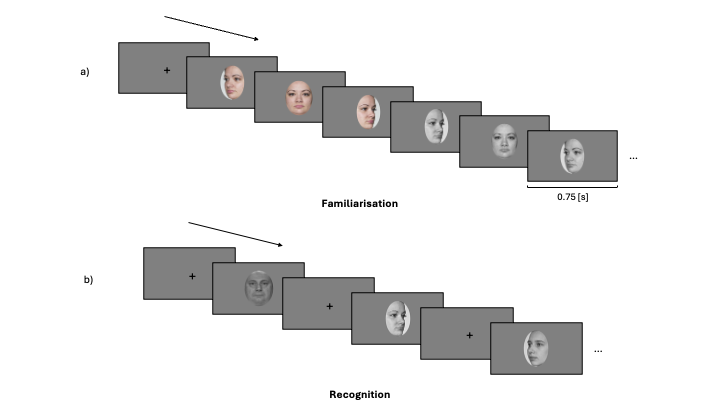
\includegraphics[keepaspectratio]{figures/Experimental_procedure_exp1.png}}

}

\caption{\label{fig-proc-exp1}Experimental procedure of Experiment 1}

\end{figure}%

\emph{The experimental procedure was divided into two parts: a
familiarization part and a recognition part. a) In the familiarization
part, participants were asked to memorize the face identity of 30
identities. For each identity, participants looked at 6 pictures
depicting the same identity with different face orientation (3/4 left
view, frontal view and 3/4 right view) and different colorimetry (color
and gray scale images) in the order presented here: 3/4 left view,
frontal view and 3/4 right view in color, followed by 3/4 right view,
frontal view and 3/4 left view in gray scale. b) In each trial of the
recognition part, participants had to decided if they recognize the face
shown on the screen from the familiarization part. If they did, they had
to press the ``q'' key and if the did not, the ``p'' key. They completed
three blocks of 60 trials (half of them were from the familiarization
part, half were novel faces). For the recognition part, only gray scale
images of faces were used (for both learned faces and novel faces).}

\subsection{Experiment 2}\label{experiment-2}

\subsubsection{Participants}\label{participants-1}

All participant were recruited on the Prolific platform
(\url{https://www.prolific.com}). Participants had to be located in the
United Kingdom or in the United States, be aged between 18-65 years old,
with normal or corrected-to-normal vision and speak fluent English.
Furthermore, Prolific offers the option to chose the approval rate of
the participants willing to take part in the study. The approval rate is
the percentage for which participants has been approved in previous
experiment. An approval rating between 95\% and 100\% was chosen in our
study to try to ensure high data quality. 35 participants completed
Experiment 2. Following our preregistered exclusion criterion, 4
participants were excluded because their percentage of missed trials was
higher than 25\% and 1 was removed because the overall accuracy was
lower than 55\%. In the end, data from 30 participants (20 men and 10
women) were retained for the analysis and the LBA modeling. Ages ranged
from 25 to 61 (\(M_{age} =\) 41.7, \(SD_{age} =\) 12). Following
Prolific payment principles, each participant received 9£ for the
completion of the study.

\subsubsection{Stimuli}\label{stimuli-1}

In an attempt to replicate the findings of Experiment 1, the stimuli
used in this experiment were exactly the same as the ones used in
Experiment 1 (See Method and Materials, Experiment 1, Stimuli).

\subsubsection{Material}\label{material-1}

Given the online nature of this experiment, participants were asked to
complete the study using a desktop computer. The experimental procedure
has been tested on three different operative systems (PC, Macintosh and
Linux), as well as on three different web browsers (Google Chrome,
Safari and Firefox). Participants were asked to specifically used these
operating systems and web browsers to ensure a consistent procedure and
participant experience.

\subsubsection{Procedure}\label{procedure-1}

On Prolific, participants who wished to take part in the experiment read
the study information and selected an URL link to the Pavlovia (Open
Science Tools, Nottingham, UK) platform. After selecting the URL link, a
Pavlovia webpage opened to the inform consent of the study. Participants
chose if they wanted to complete this study or not after reading the
inform consent. The access to the task was only granted if participants
accepted the terms of the inform consent.

Regarding the experimental procedure, it was almost identical to the one
used in Experiment 1 (Method and Materials, Experiment 1, Procedure). A
response time window was added in the recognition part of the
experiment. Instead of removing trials with a response time higher than
2.5 seconds after data collection, we decided to implement a response
time window of 2 seconds for each recognition trial. In Experiment 1,
13.796\% of the trials were longer than 2 seconds. We expected
participants to quickly get accustomed to the response time limit and
that the average percentage of missed trials will be similar or lower
than in Experiment 1. Response time {[}s{]} and accuracy were collected
after each recognition trial.

\subsection{Experiment 3}\label{experiment-3}

\subsubsection{Participants}\label{participants-2}

All participant were recruited using either an online recruiting
platform (\url{https://marktplatz.uzhalumni.ch}) or via a mailing list
dedicated to students from the Department of Psychology of the
University of Zurich. 40 healthy participants completed Experiment 3. We
deviated from our preregistration in one way. Since this experiment was
conducted to investigate how highly familiar faces affect the
computational processes of face recognition, we had to remove 9 more
participants who did not show a level of familiarity high enough with
the presented faces in the first part of the experiment. This scenario
did not occur during the pilot experiments we conducted and thus was not
part of our preregistration.

Based on our preregistered criteria, a further participant was excluded
from further data analysisdue to an overall recognition accuracy larger
than 95\%. In the end, the data of 30 participants (13 men and 17 women)
were retained for further analysis and LBA modeling. Ages ranged from 20
to 42 years old (\(M_{age} =\) 26.8, \(SD_{age} =\) 5.8). All
participants reported normal or corrected-to-normal vision and received
payment (25 CHF) for participating in the experiment.

\subsubsection{Stimuli}\label{stimuli-2}

Two types of pictures were used for this experiment to create our
within-subject stimuli conditions. Images used for the ``Novel''
condition were the same pictures used in Experiment 1: the data set of
face images contained 378 images since only the set of three gray scaled
face images for each of the 126 identities was used for this experiment.
Pictures depicting celebrities (``Famous'' condition) were taken from
the internet. For each of the 60 preselected celebrities, 3 pictures
depicting them from a similar angle to the ``Novel'' faces were chosen
(3/4 left view, frontal view and 3/4 right vie). Moreover, 60 more
pictures (one for each of the celebrities) was only used for the first
part of the experiment. All of the ``Famous'' images processing was
realized using the GNU Image Manipulation Program (The GIMP Development
Team (2025)). Background was removed from the picture and replace by the
same background used in the ``Novel'' images. The same gray scale filter
used for the ``Novel'' faces was applied to the celebrities images used
during the recognition part. In total, the data set of face images used
in this experiment contained 618 images: 1 set of three gray scaled face
images for each of the 126 novel identities, 1 set of three gray scaled
face images for each of the 60 famous identities and 60 images of
celebrities used in the first part of the experiment. Furthermore, a
gray mask was added on top of each pictures (``Novel'' faces and
``Learned'' faces) during the recognition part. Each mask was composed
of 10 grey rectangles which position differs in function of the face
orientation (See Figure~\ref{fig-mask-exp3} for an example of the mask
in question). The addition of a grey mask on top the face images
decreased the overall accuracy of the recognition part during pilot work
to a percentage of correct answer suited for the application of
evidence-accumulation modeling.

\begin{figure}

\centering{

\pandocbounded{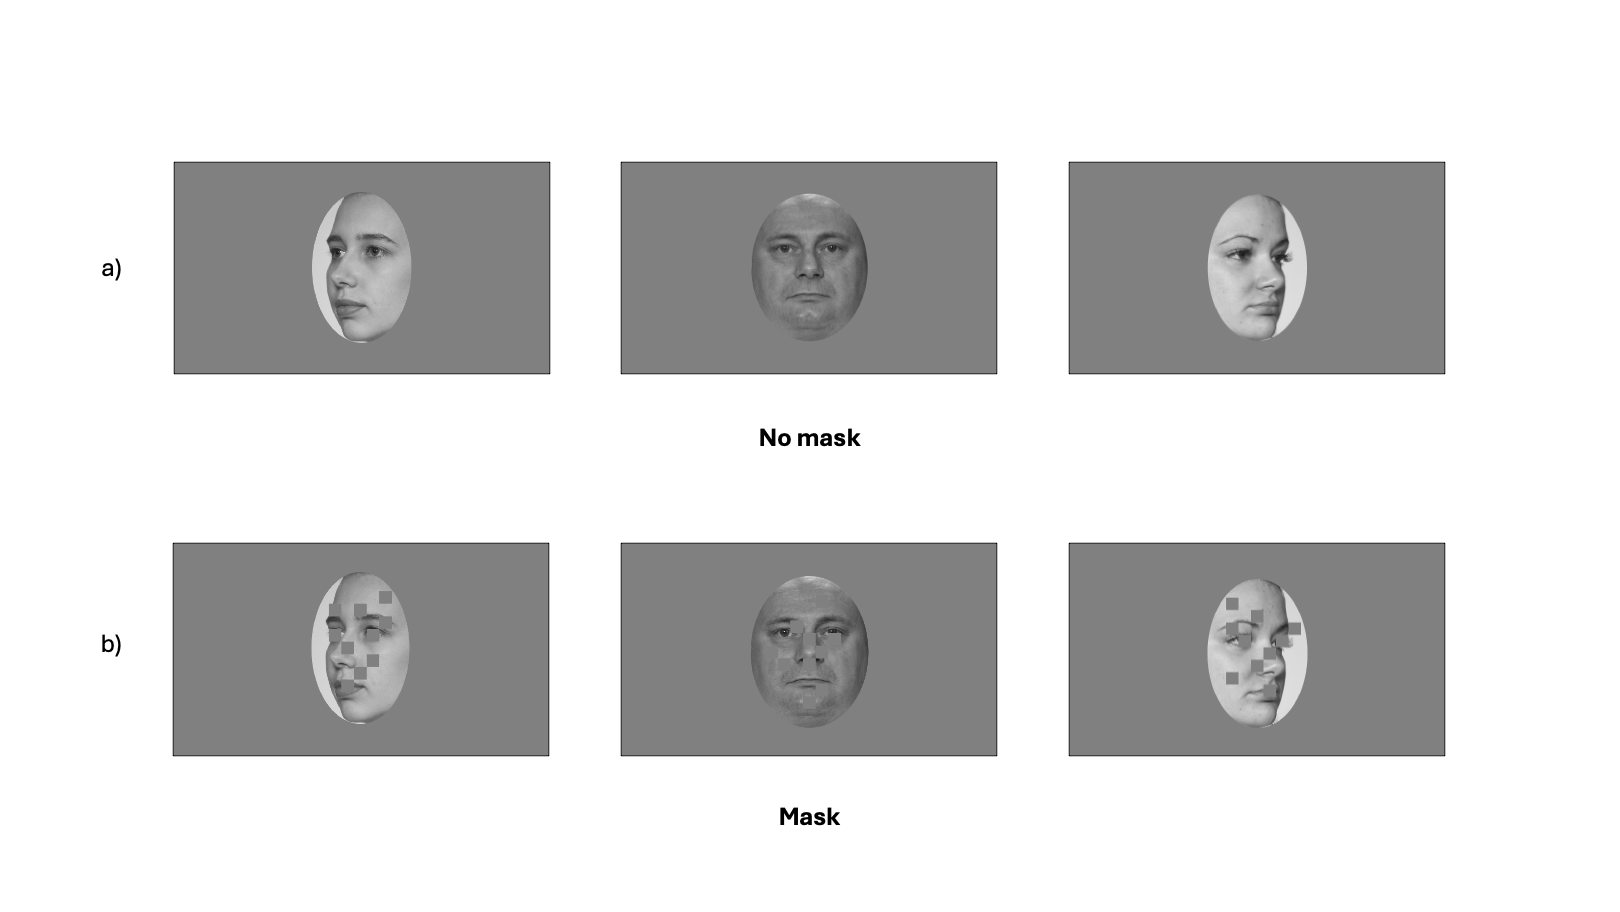
\includegraphics[keepaspectratio]{figures/Mask_exp3.png}}

}

\caption{\label{fig-mask-exp3}Non-masked and masked images}

\end{figure}%

\emph{a) Images showing faces used in Experiment 1 and 2 for the three
different face orientation (3/4 left, frontal view, 3/4 right) b) Same
faces with the gray mask added on top of the images. These images were
used in the recognition part of Experiment 3. Each mask is composed of
10 gray rectangles which position was adapted in function of the face
orientation.These faces were used in the ``novel'' condition of
Experiment 3.}

\subsubsection{Material}\label{material-2}

Stimuli were presented on the screen of a MacBook Pro (Apple M2 Pro,
macOS 14 Sonoma). The experiment was run on Psychopy Coder (version:
2022.5, Peirce et al. (2019)) and the code used for the experimental
procedure is available on OSF (\url{https://osf.io/ut78f/overview}).

\subsubsection{Procedure}\label{procedure-2}

The experimental task was divided into two distinct parts: a rating part
and a recognition part (Figure~\ref{fig-proc-exp3}). During the rating
part, participants were presented pictures of 60 celebrities. They were
asked to rate these celebrities on two different features: how familiar
the celebrity was to them (from 0: Highly unfamiliar to 10: Highly
familiar) and how positive or negative were their feelings towards the
celebrity (from 0:Highly negative to 10: Highly positive). After the two
rating scales, participants were asked to choose the correct name of the
same identity from four different naming options. From the 60
celebrities faces presented during the rating part, the 30 celebrities
with the highest familiarity (with a minimum of 7 out of 10) and whose
names were correctly assigned were for the ``Famous'' faces condition of
the recognition part. Thus, the set of ``Famous'' faces used in the
recognition part was individualized for each participant. In the
recognition part, participants completed three blocks of 90 recognition
trials. Each block was separated from another by a short break. Half of
the trials were famous identities trials and the other half were new,
previously unseen identities trials. At each trial, a gray scale image
of a face was shown on the screen. Participants were asked to choose if
they recognize the face (and not the picture) seen this face in the
familiarization part or not. If they did, the should press the ``q'' key
and if they did not, the ``p'' key. Based on pilot work, task difficulty
was increased by adding a response time window of 0.9 second during each
recognition trial. Response time {[}s{]} and accuracy were collected
after each trial.

\begin{figure}

\centering{

\pandocbounded{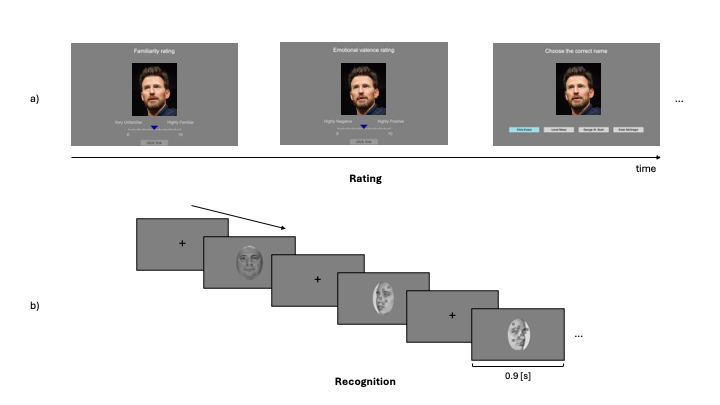
\includegraphics[keepaspectratio]{figures/Experimental_procedure_exp3.png}}

}

\caption{\label{fig-proc-exp3}Experimental procedure of Experiment 3}

\end{figure}%

\emph{The experimental procedure was divided into two parts: a rating
part and a recognition part. a) In the rating part, participants were
asked to rate famous faces on two distinct features using rating scales
(0-10): their familiarity (low to high) and the emotional valence
(negative to positive). After the two rating scales, they had to chose
the correct name of the celebrities from four different naming
options.(Disclaimer: the picture used here was not used in the actual
rating part of the experiment. Its purpose here is to demonstrate what
participants had to realize in the first part of the experiment. Image
attribution: Philip Romano, CC BY-SA 4.0
\url{https://creativecommons.org/licenses/by-sa/4.0}, via Wikimedia
Commons,
\url{https://commons.wikimedia.org/wiki/File:ChrisEvans2023.jpg}) b) In
each trial of the recognition part, participants had to decided if they
recognize the face shown on the screen. If they did, they had to press
the ``q'' key and if the did not, the ``p'' key. They completed three
blocks of 60 trials (half of them were famous faces, half were novel
faces).}

\subsubsection{Issues with response times
collection}\label{issues-with-response-times-collection}

During data analysis, we observed that the distribution of the response
times for Experiment 3 looked did not look positively skewed (right
skewed). After investigation of the code used to run the experiment, we
noticed that there was a coding error, which resulted in this abnormal
response times distribution. We decided to not run further data analysis
(LBA model) for this experiment because evidence-accumulation models
expect the response times distribution to be right skewed. Instead, we
decided to replicate Experiment 4, in which the same face familiarity
levels (novel vs famous) were manipulated.

\subsection{Experiment 4 and Experiment
5}\label{experiment-4-and-experiment-5}

\subsubsection{Participants}\label{participants-3}

All participant were recruited on the Prolific platform
(\url{https://www.prolific.com}) using the same criteria as Experiment
2.

For Experiment 4, 46 participants completed the experiment. Following
our preregistered exclusion criterion, 12 did not show a sufficiently
high level of familiarity with the famous faces. In addition, 1
participant was excluded because the percentage of missed trials was
higher than 25\% and 3 were removed because the overall accuracy was
lower than 55\% or higher than 95\%. In the end, the data of 30
participants (17 men and 13 women) were retained for further analysis
and LBA modeling. Ages ranged from 25 to 61 (\(M_{age} =\) 39.5,
\(SD_{age} =\) 10). Following Prolific payment principles, each
participant received 9£ for the completion of the study.

46 participants completed Experiment 5. 12 did not show a sufficiently
high level of familiarity with the famous faces and 3 were removed
because the overall accuracy was lower than 55\% or higher than 95\%. In
the end, the data of 31 participants (14 men and 17 women) were retained
for further analysis and LBA modeling. Ages ranged from 18 to 59
(\(M_{age} =\) 37.4, \(SD_{age} =\) 10.9). Following Prolific payment
principles, each participant received 9£ for the completion of the
study.

\subsubsection{Stimuli}\label{stimuli-3}

Initially, we planned to use the exact same stimuli as the one used in
Experiment 3. However, during the pilot, it was noticed that the
``Famous'' faces and the ``Novel'' faces contained differences in low
visual features such as brightness, luminosity angle and the resolution
of the picture. These differences might have aided the categorization
between ``famous'' and ``novel'' stimuli and affected the estimation of
our parameters of interest. To avoid that decisions are based on visual
features and not on familiarity, we changed the face pictures data set
for both conditions in Experiment 4 and Experiment 5.

For the ``Famous'' condition, faces were all taken from
\url{https:://commons.wikimedia.org}. For each of the famous identities
(30 men, 30 women), four pictures were selected: one for the rating part
of the experiment and three were used in the recognition part. The list
of the attributions as well as the URL links to all the pictures can be
found on OSF (\url{https://osf.io/65bt2/overview}). For the ``Novel''
condition, face images were taken from the ``10K US Adult Faces
Database'' (Bainbridge et al., 2013). These pictures depict faces in a
natural environment, similar to the selected images of the celebrities.
103 faces were selected from this database and used in the recognition
part of the experiment.

To avoid recognition based on low visual features, we decided to not
standardize the brightness and luminosity angle of the entire picture
dataset for both novel and famous faces. The original viewing point,
luminosity angle, brightness and background of the picture were not
manipulated. The rationale behind this decision was to avoid adding
modifications to the original image that might facilitate the
categorization between the stimuli conditions. The only low level visual
feature that we standardized across all the images was the resolution.
After cropping, every images was down sampled to a 250 pixels (px)
height, a height similar to the original height of the images from ``10K
US Adult Faces Database'', and grayscaled.

\subsubsection{Material}\label{material-3}

As Experiment 2, since this was an online data collection protocol,
participants were asked to complete the study using a desktop computer.

\subsubsection{Procedure}\label{procedure-3}

The online procedure was the same as the one described for Experiment 2:
on Prolific, participants who wished to take part in the experiment read
the study information and selected an URL link to the Pavlovia platform.
After selecting the URL link, a Pavlovia webpage opened to the inform
consent of the study. Participants chose if they wanted to complete this
study or not after reading the inform consent. The access to the task
was only granted if participants accepted the terms of the inform
consent.

The experimental procedure was similar to the one used for Experiment 3
(see Method and Materials, Experiment 3, Procedure): participants first
underwent a rating part which preceded the recognition part. The only
modification added to the recognition part was the increase of the
response time window from 0.9s to 1.1s.

\subsection{Evidence accumulation
modeling}\label{evidence-accumulation-modeling}

\subsubsection{Model specification}\label{model-specification}

A hierarchical LBA model was fit to the data with model specifications
outlined in our preregistrations (Table~\ref{tbl-model-formula}). LBA
models have one accumulator for each response option, with potentially
different parameter values. In our design, that meant that for
Experiment 1 and 2, there was one accumulator for the ``Learned''
response and another for the ``Novel'' response. For Experiment 4 and 5,
there was one accumulator for the ``Famous'' response and another for
the ``Novel'' response. More specifically, for Experiment 1 and 2,
threshold was allowed to vary by participants' response (Learned/Novel)
whereas mean drift rate was allowed to vary by the stimulus condition
(Learned/Novel) and the match between the accumulator and the stimulus
(TRUE/FALSE). If the stimulus was ``Learned'', then the accumulator for
the ``Learned'' response would be TRUE, whereas the accumulator for the
``Novel'' response would be FALSE. The difference between the TRUE and
FALSE accumulator represents the quality of the information processing
about a decision (Lewandowsky \& Oberauer, 2018). A greater difference
between these accumulators means a greater quality of evidence
accumulating towards that decision.

For every model, threshold was allowed to vary by response
(Novel/Learned for Experiment 1 and 2, Novel/Famous for Experiment 4 and
5). The standard deviation for the true accumulator was allowed to vary
by the match factor whereas the the standard deviation for the false
accumulator was kept uniform to make the model identifiable (Donkin et
al., 2009). A single value for the start point (A) and non-decision time
(t0) was estimated for our preregistered models but model estimations
where these parameters were allowed to vary are described in
supplementary materials.

\begin{table}

\caption{\label{tbl-model-formula}Formula specification for the
pre-registered linear ballistic accumulator model.}

\centering{

\centering
\begin{talltblr}[         %% tabularray outer open
entry=none,label=none,
note{}={Condition = training condition (Learned vs. Novel or Famous vs. Novel); Response = key-press response (same vs. different); Accuracy = (true/correct vs false/incorrect); SD = standard deviation.},
]                     %% tabularray outer close
{                     %% tabularray inner open
colspec={Q[]Q[]Q[]Q[]Q[]Q[]},
hline{2}={1-6}{solid, black, 0.05em},
hline{1}={1-6}{solid, black, 0.08em},
hline{8}={1-6}{solid, black, 0.08em},
}                     %% tabularray inner close
Parameter & Label & Condition & Response & Accuracy & Fixed \\
Start point & A & - & - & - & - \\
Mean drift rate & v & yes & no & yes & - \\
SD drift rate & sd_v & no & no & yes & - \\
SD false drift rate & false.sd_v & - & - & - & 1 \\
Threshold & b & no & yes & no & - \\
Non-decision time & t0 & - & - & - & - \\
\end{talltblr}

}

\end{table}%

\subsubsection{Model estimation}\label{model-estimation}

We carried out a Bayesian model estimation using the EMC2 R package.
Details about the priors of each model are provided in supplementary
materials and the code required to run the analyses is available on OSF.
Priors were chosen to be weakly-informative meaning that they have
little influence on the estimation. The parameter were estimated through
two sampling steps. First, a separate estimation of the fixed effects
for each participants was conducted. These estimations were used as the
starting point for the full hierarchical model. Chains convergence
diagnostics, as well as priors distributions and predictive checks can
be found in Supplementary Materials.

\subsubsection{Data analysis}\label{data-analysis}

For every experiment, the separate analysis of response times and
accuracy was conducted using Bayesian Multilevel Models with R Package
brms (Bürkner, 2017). The evidence-accumulation modelling analyses of
the distributions of response times for the correct and wrong answers
were realized using the EMC2 R package (Stevenson et al., 2025). In
order to make inference about the magnitude of familiarity effects,
differences in parameter estimates across conditions were compared. Our
inferences are based on the median and 95\% quantile interval of the
posterior distributions and the difference contrasts between the
conditions of interest.

\section{Results}\label{results}

First, we show raw data plots and descriptive statistics when reaction
time and accuracy are analyses separately. Second, results from the LBA
modeling will be presented.

\subsection{Raw data plots and descriptive
statistics}\label{raw-data-plots-and-descriptive-statistics}

\begin{figure}

\begin{minipage}[t]{\linewidth}

\centering{

\pandocbounded{
\includegraphics[keepaspectratio]{manuscript_files/figure-latex/fig-acc-rt-1.png}}

}

\subcaption{\label{fig-acc-rt-1}Proportion of correct responses
{[}\%{]}}

\end{minipage}%
\newline
\begin{minipage}[t]{\linewidth}

\centering{

\pandocbounded{
\includegraphics[keepaspectratio]{manuscript_files/figure-latex/fig-acc-rt-2.png}}

}

\subcaption{\label{fig-acc-rt-2}Mean response times {[}s{]}}

\end{minipage}%

\caption{\label{fig-acc-rt}Proportion of correct responses {[}\%{]} and
mean response times {[}s{]} across conditions for the four experiments.
Coloured points represent individual participant averages, black points
denote the group mean and error bars represent 95\% confidence
intervals.}

\end{figure}%

\begin{figure}

\centering{

\pandocbounded{
\includegraphics[keepaspectratio]{manuscript_files/figure-latex/fig-rt-density-1.png}}

}

\caption{\label{fig-rt-density}Density of response times {[}s{]} across
conditions for the four experiments. The density plot for Experiment 3
clearly shows the timing quantisation artefact discussed in the Methods,
where keypress responses were recorded in \textasciitilde80ms bins
rather than continuously.}

\end{figure}%

\subsection{Evidence accumulation modeling
results}\label{evidence-accumulation-modeling-results}

For all experiments, posterior distributions for drift rate and
threshold parameters are visualised in Figure~\ref{fig-threshold-all}
and Figure~\ref{fig-drift-all} and the medians and 95\% quantile
intervals are summarised in Table~\ref{tbl-lba-params}.

\subsubsection{Experiment 1}\label{experiment-1-1}

\emph{Threshold:} We estimated the threshold parameter for both response
options (Novel and Learned). Inspection of the posterior distributions
of the effect of face familiarity on the threshold parameter shows that
while the threshold for Novel faces is greater that the one for Learned
faces.

\begin{figure}

\begin{minipage}[t]{0.50\linewidth}

\centering{

\pandocbounded{
\includegraphics[keepaspectratio]{manuscript_files/figure-latex/fig-threshold-all-1.png}}

}

\subcaption{\label{fig-threshold-all-1}Threshold by response}

\end{minipage}%
%
\begin{minipage}[t]{0.50\linewidth}

\centering{

\pandocbounded{
\includegraphics[keepaspectratio]{manuscript_files/figure-latex/fig-threshold-all-2.png}}

}

\subcaption{\label{fig-threshold-all-2}Threshold contrast}

\end{minipage}%

\caption{\label{fig-threshold-all}Threshold estimates across
experiments}

\end{figure}%

\emph{Drift rate:} To quantify the contribution of face familiarity on
the drift rate, we computed the difference between the TRUE and FALSE
drift rate for each familiarity condition as our main dependent measure.
To estimate the familiarity effect, we then subtracted the drift rate
difference on learned trials from novel trials. Inspection of the
posterior distribution shows that there is a novelty effect in drift
rate difference in Experiment 1. The quality of the evidence
accumulation was greater for Novel faces compared to Learned faces.

\begin{figure}

\begin{minipage}[t]{0.50\linewidth}

\centering{

\pandocbounded{
\includegraphics[keepaspectratio]{manuscript_files/figure-latex/fig-drift-all-1.png}}

}

\subcaption{\label{fig-drift-all-1}Drift rate (TRUE - FALSE) by
condition}

\end{minipage}%
%
\begin{minipage}[t]{0.50\linewidth}

\centering{

\pandocbounded{
\includegraphics[keepaspectratio]{manuscript_files/figure-latex/fig-drift-all-2.png}}

}

\subcaption{\label{fig-drift-all-2}Drift rate contrast}

\end{minipage}%

\caption{\label{fig-drift-all}Drift rate estimates across experiments}

\end{figure}%

\begin{table}

\caption{\label{tbl-lba-params}Posterior median and 95\% quantile
intervals for threshold and drift rate parameters across experiments.}

\centering{

\centering
\begin{talltblr}[         %% tabularray outer open
entry=none,label=none,
note{}={QI = quantile interval.},
]                     %% tabularray outer close
{                     %% tabularray inner open
colspec={Q[]Q[]Q[]Q[]},
hline{2}={1-4}{solid, black, 0.05em},
hline{1}={1-4}{solid, black, 0.08em},
hline{30}={1-4}{solid, black, 0.08em},
column{2-4}={}{font=\fontsize{0.85em}{1.15em}\selectfont},
row{1,3,4,5,6,7,8,10,11,12,13,14,15,17,18,19,20,21,22,24,25,26,27,28,29}={}{font=\fontsize{0.85em}{1.15em}\selectfont},
cell{2,9,16,23}{1}={c=4}{font=\fontsize{0.85em}{1.15em}\selectfont},
}                     %% tabularray inner close
Parameter & Condition & Median & 95% QI \\
Experiment 1 & Experiment 1 & Experiment 1 & Experiment 1 \\
Threshold & novel & 1.45 & [1.278, 1.628] \\
Threshold & learned & 1.33 & [1.163, 1.5] \\
Threshold contrast & novel - learned & 0.12 & [0.022, 0.219] \\
Drift rate & novel & 2.11 & [1.922, 2.31] \\
Drift rate & learned & 0.77 & [0.626, 0.914] \\
Drift rate contrast & novel - learned & 1.35 & [1.074, 1.618] \\
Experiment 2 & Experiment 2 & Experiment 2 & Experiment 2 \\
Threshold & novel & 1.82 & [1.639, 2.013] \\
Threshold & learned & 1.49 & [1.331, 1.664] \\
Threshold contrast & novel - learned & 0.33 & [0.233, 0.433] \\
Drift rate & novel & 1.3 & [1.156, 1.449] \\
Drift rate & learned & 0.24 & [0.094, 0.381] \\
Drift rate contrast & novel - learned & 1.06 & [0.806, 1.323] \\
Experiment 4 & Experiment 4 & Experiment 4 & Experiment 4 \\
Threshold & novel & 2.36 & [2.144, 2.565] \\
Threshold & famous & 1.67 & [1.518, 1.82] \\
Threshold contrast & novel - famous & 0.69 & [0.561, 0.816] \\
Drift rate & novel & 2.76 & [2.541, 2.986] \\
Drift rate & famous & -0.16 & [-0.361, 0.044] \\
Drift rate contrast & novel - famous & 2.92 & [2.53, 3.32] \\
Experiment 5 & Experiment 5 & Experiment 5 & Experiment 5 \\
Threshold & novel & 2.29 & [2.135, 2.45] \\
Threshold & famous & 1.72 & [1.594, 1.841] \\
Threshold contrast & novel - famous & 0.58 & [0.479, 0.679] \\
Drift rate & novel & 2.16 & [1.983, 2.34] \\
Drift rate & famous & -0.05 & [-0.227, 0.113] \\
Drift rate contrast & novel - famous & 2.21 & [1.888, 2.546] \\
\end{talltblr}

}

\end{table}%

\subsubsection{Experiment 2}\label{experiment-2-1}

\emph{Threshold:} Inspection of the posterior distribution shows that
there is an effect of familiarity on the threshold parameter.

\emph{Drift rate:} Inspection of the posterior distribution shows that
there is a similar familiarity effect in drift rate difference as in
Experiment 1. The quality of the evidence accumulation was greater for
Novel faces compared to Learned faces.

\subsubsection{Experiment 3}\label{experiment-3-1}

As explained in the Methods, due to a timing artefact in data collection
(responses recorded in discrete 80ms bins), the RT distributions from
Experiment 3 do not meet the continuity assumptions of the LBA and we do
not report model parameter estimates for this experiment.

\subsubsection{Experiment 4}\label{experiment-4}

\emph{Threshold:} Inspection of the posterior distribution shows that
there is an effect of familiarity on the threshold parameter. Threshold
was greater for Novel faces than for Famous faces.

\emph{Drift rate:} Inspection of the posterior distribution shows that
there is a familiarity effect in drift rate difference, which mirrors
the results from Experiment 1 and Experiment 2. The quality of the
evidence accumulation was greater for Novel faces compared to Famous
faces.

\subsubsection{Experiment 5}\label{experiment-5}

\emph{Threshold:} Inspection of the posterior distribution shows that
there is an effect of familiarity on the threshold parameter which
mirrors the results from Experiment 4.

\emph{Drift rate:} Inspection of the posterior distribution shows that
there is a familiarity effect in drift rate difference, which mirrors
the results from Experiment 1, Experiment 2 and Experiment 4. The
quality of the evidence accumulation was greater for Novel faces
compared to Famous faces.

\section{General discussion}\label{general-discussion}

We set out to understand not merely \emph{that} familiarity affects face
recognition, but \emph{how} --- specifically, which latent computational
processes are modulated when a face is familiar versus novel. By fitting
linear ballistic accumulator models to recognition data across a series
of experiments, we show that familiarity primarily affects the quality
of evidence accumulation, with a secondary and smaller effect on
response caution. This computational signature --- a novelty advantage
in drift rate, accompanied by a modest novelty advantage in threshold
--- replicates across visual familiarity (Experiments 1 and 2), and
visual familiarity and person knowledge (Experiment 4 and 5). These
findings move beyond manifest measures of accuracy and response time to
characterise the decision-level mechanisms that underpin familiar face
recognition (Phillips \& White, 2025).

\subsection{The impact of visual
familiarity}\label{the-impact-of-visual-familiarity}

The most theoretically important finding is the combination of drift
rate and threshold effects. Across Experiments 1 and 2, the novelty
advantage in drift rate was substantially larger than the novelty
advantage in threshold. This dissociation matters because the two
parameters reflect qualitatively different aspects of the decision
process. Drift rate indexes the quality of evidence accumulation --- how
cleanly and rapidly perceptual and cognitive systems extract
decision-relevant information from a face. Threshold indexes how much
accumulated evidence is required before a decision is triggered. The
dominance of the drift rate effect localises familiarity's influence to
the quality of signal from the image more so than as a function of
response bias between novel and familiar key presses.

Set within the Bruce and Young framework of face perception (Bruce \&
Young, 1986), visual familiarity modulates the quality of structural
encoding and feature matching within the core face processing system
(Bruce \& Young, 1986; Gobbini \& Haxby, 2006), thus generating a
stronger perceptual signal that feeds into the decision process. One
interpretation of the pattern of results obtained here could be that
novel faces, by this account, provide a cleaner and less ambiguous
perceptual signal than visually familiar faces --- consistent with
``pop-out'' and attentional capture accounts (W. A. Johnston et al.,
1990; Lev-Ari et al., 2022; Lubow \& Kaplan, 1997). In contrast,
visually familiar faces may generate noisier representations due to
interference from accumulated but imperfectly consolidated memory traces
(Rapcsak, 2019).

The smaller but reliable threshold effect reflects a qualitatively
different influence on performance. In a yes/no recognition task,
participants must set separate response criteria for the ``familiar''
and ``novel'' responses, and the higher threshold for the novel response
is consistent with a well-documented conservative rejection bias in
recognition memory (Glanzer \& Adams, 1985; Stretch \& Wixted, 1998):
participants are more willing to endorse familiarity than to endorse
novelty, requiring more evidence before committing to a rejection.
Because the drift rate advantage is substantially larger, the net
behavioural outcome remains a novel face advantage in speed and accuracy
--- the signal quality benefit outweighs the response caution cost.

\subsection{The impact of person
knowledge}\label{the-impact-of-person-knowledge}

Extending these findings to person knowledge is theoretically important
because famous faces engage not only the core face processing system but
also the extended system, which mediates retrieval of identity-specific
person knowledge (Duchaine \& Yovel, 2015; Gobbini \& Haxby, 2007).
Experiment 4 and 5 showed a pattern broadly consistent with Experiments
1 and 2: novel faces produced higher drift rates and slightly higher
response caution than famous faces. This raises the possibility that the
computational signature of novelty generalises beyond visual familiarity
to person knowledge contexts. Moreover, the effects were larger for
drift rate and threshold compared to Experiments 1 and 2, which might
suggest that the more stable memory traces for famous people based on
the added person knowledge could exaggerate the novelty or ``pop-out''
effect.

At this stage, however, we remain cautious in our conclusion here and
suggest that person knowledge effects on drift rate and threshold remain
a largely open empirical question, which requires careful further
investigation using improved and/or different stimuli, such as
personally familiar people (e.g., family, friends or partners). More
generally, our findings underscore that although the study of true
familiarity - where person knowledge is available - is more akin to our
real-world experiences of interacting with familiar people, it is
inherently more difficult to study with tight experimental control
(Burton, 2024).

\subsection{Limitations}\label{limitations}

A novelty advantage in drift rate is in conceptual agreement with
studies that reported a better perception ability for novel faces than
for visually familiar faces (Bindemann et al., 2014; Read \& Hammersley,
1990), whist being in apparent tension with prior work reporting better
recognition performance for famous or personally familiar faces (Hancock
et al., 2000; Jenkins \& Burton, 2011; Klatzky \& Forrest, 1984). We
suggest two factors may contribute to this discrepancy. First, prior
studies used manifest measures that conflate signal quality with
response bias, which makes interpretation more difficult (Wagenmakers et
al., 2007). Second, novel faces may benefit from a processing advantage
specific to the task structure (old/new detection task): a correct novel
response requires only the absence of a recognition signal, whereas a
correct famous response requires the presence of one. However, using
this design also has benefits as it allows comparison to numerous
previous works that did use an old/new recognition task with faces or
other stimuli to study visual recognition. Whether the novelty advantage
in drift rate reflects a genuine signal quality effect, a task
asymmetry, or both, remains an open question that future work should
address by comparing LBA parameters across paradigms that vary the
demands placed on novel versus familiar face processing.

Previous evidence accumulation model development studies have emphasised
how the number of trials per cell of the design can influence model
fitting and parameter estimation (Alexandrowicz \& Gula, 2020; Lerche et
al., 2017; Wagenmakers et al., 2007). Our design (90 trials per
condition) and control of error rates followed the minimum
recommendations to apply EAM (Lüken et al., 2025), as well as a
parameter recovery study that showed 90 trials per condition was
sufficient to recover simulated parameters. Practical considerations
were also incorporated, including the challenge of finding face stimuli
with standardized low-level visual features that includes a large number
of identities. Nonetheless, adding more trials per condition (e.g., 200
per condition; {Boag et al.} (2025)) would have increased the robustness
of our parameter estimates.

\subsection{Future directions}\label{future-directions}

We can think of several relevant future directions in addition to the
ones already mentioned. First, a learning curve design that tracks LBA
parameters across repeated exposure sessions would address at which
stage of familiarity drift rate changes occur, and would provide a more
dynamic account of how computational processes change as familiarity is
acquired (Ramon \& Gobbini, 2018). Second, to more directly link
together computational processes and neural architectures, future
research might use a joint-modelling approach (Palestro et al., 2018; Vo
et al., 2024). Joint-modelling integrates different sources of data
(e.g.~behavioural and neuroimaging data) to estimate the relationship
between responses in particular brain regions, such as core and extended
face networks, and latent computational parameters. Third, individual
differences in face recognition ability represent a natural and
important extension. Super-recognisers and individuals with
developmental prosopagnosia differ dramatically in recognition
performance (Dobel et al., 2007; Duchaine \& Nakayama, 2006; Russell et
al., 2009), and drift rate --- as the primary carrier of familiarity
effects here --- may be the parameter that most cleanly differentiates
these groups. Fourth, testing the domain-specificity of these effects
would be valuable to determine whether the effects of visual familiarity
apply to other categories of visual stimuli, such as objects or scenes.

\newpage{}

\section{Disclosures}\label{disclosures}

\subsection{Data and code
availability}\label{data-and-code-availability}

All materials are available on GitHub (link) and the OSF (link).

\subsection{Author contributions}\label{author-contributions}

\href{https://www.elsevier.com/researcher/author/policies-and-guidelines/credit-author-statement}{CRediT}
author statement:

Conceptualization: RF, PD, RR\\
Data Curation:RF, RR\\
Formal Analysis: RF, RR\\
Funding Acquisition: RR\\
Investigation: RF\\
Methodology: RF, RR\\
Project Administration: RF, RR\\
Resources: RR\\
Software: RF, RR\\
Supervision: RR\\
Validation: RF, RR\\
Visualisation: RF, RR\\
Writing - Original Draft: RF\\
Writing - Review \& Editing: RF, PD, RR\\

\subsection{Competing interests}\label{competing-interests}

The authors declare no competing interests.

\newpage{}

\section{References}\label{references}

\protect\phantomsection\label{refs}
\begin{CSLReferences}{1}{0}
\bibitem[\citeproctext]{ref-akanHaventSeenYou2023}
Akan, M., \& Benjamin, A. S. (2023). Haven't i seen you before?
Conceptual but not perceptual prior familiarity enhances face
recognition memory. \emph{Journal of Memory and Language}, \emph{131},
104433. \url{https://doi.org/10.1016/j.jml.2023.104433}

\bibitem[\citeproctext]{ref-alexandrowiczComparingEightParameter2020}
Alexandrowicz, R. W., \& Gula, B. (2020). Comparing eight parameter
estimation methods for the ratcliff diffusion model using free software.
\emph{Frontiers in Psychology}, \emph{11}, 484737.
\url{https://doi.org/10.3389/fpsyg.2020.484737}

\bibitem[\citeproctext]{ref-bainbridgeIntrinsicMemorabilityFace2013}
Bainbridge, W. A., Isola, P., \& Oliva, A. (2013). The intrinsic
memorability of face photographs. \emph{Journal of Experimental
Psychology: General}, \emph{142}(4), 1323--1334.
\url{https://doi.org/10.1037/a0033872}

\bibitem[\citeproctext]{ref-bindemannPerceivedAbilityActual2014}
Bindemann, M., Attard, J., \& Johnston, R. A. (2014). Perceived ability
and actual recognition accuracy for unfamiliar and famous faces.
\emph{Cogent Psychology}, \emph{1}(1), 986903.
\url{https://doi.org/10.1080/23311908.2014.986903}

\bibitem[\citeproctext]{ref-birdEffectsPreexperimentalKnowledge2011}
Bird, C. M., Davies, R. A., Ward, J., \& Burgess, N. (2011). Effects of
pre-experimental knowledge on recognition memory. \emph{Learning \&
Memory}, \emph{18}(1), 11--14. \url{https://doi.org/10.1101/lm.1952111}

\bibitem[\citeproctext]{ref-boagExpertGuidePlanning2025}
{Boag, R. J., Innes, R. J., Stevenson, N., Bahg, G., Busemeyer, J. R.,
Cox, G. E., Donkin, C., Frank, M. J., Hawkins, G. E., Heathcote, A., \&
al., et}. (2025). An expert guide to planning experimental tasks for
evidence-accumulation modeling. \emph{Advances in Methods and Practices
in Psychological Science}, \emph{8}(2), 25152459251336127.
\url{https://doi.org/10.1177/25152459251336127}

\bibitem[\citeproctext]{ref-brownSimplestCompleteModel2008}
Brown, S. D., \& Heathcote, A. (2008). The simplest complete model of
choice response time: Linear ballistic accumulation. \emph{Cognitive
Psychology}, \emph{57}(3), 153--178.
\url{https://doi.org/10.1016/j.cogpsych.2007.12.002}

\bibitem[\citeproctext]{ref-bruceUnderstandingFaceRecognition1986}
Bruce, V., \& Young, A. (1986). Understanding face recognition.
\emph{British Journal of Psychology}, \emph{77}(3), 305--327.
\url{https://doi.org/10.1111/j.2044-8295.1986.tb02199.x}

\bibitem[\citeproctext]{ref-brms}
Bürkner, P.-C. (2017). \emph{{\textbraceleft}Brms{\textbraceright}: An
{\textbraceleft}r{\textbraceright} package for
{\textbraceleft}bayesian{\textbraceright} multilevel models using
{\textbraceleft}stan{\textbraceright}}. \emph{80}.
\url{https://doi.org/10.18637/jss.v080.i01}

\bibitem[\citeproctext]{ref-burtonFacePerception2024}
Burton, A. M. (2024). Face perception. In \emph{Open encyclopedia of
cognitive science} (1st ed.). MIT Press.
\url{https://doi.org/10.21428/e2759450.57de91a4}

\bibitem[\citeproctext]{ref-charpentierApplicationComputationalModels2018}
Charpentier, C. J., \& O'Doherty, J. P. (2018). The application of
computational models to social neuroscience: Promises and pitfalls.
\emph{Social Neuroscience}, \emph{13}(6), 637--647.
\url{https://doi.org/10.1080/17470919.2018.1518834}

\bibitem[\citeproctext]{ref-cheongComputationalModelsSocial2017}
Cheong, J. H., Jolly, E., Sul, S., \& Chang, L. J. (2017). Computational
models in social neuroscience. \emph{Computational Models of Brain and
Behavior}, 229--244.

\bibitem[\citeproctext]{ref-debruinefacelab2017}
DeBruine, L., \& Jones, B. (2017). \emph{Face research lab london set}
(Version 5) {[}Dataset{]}. figshare.
\url{https://doi.org/10.6084/m9.figshare.5047666.v5}

\bibitem[\citeproctext]{ref-dobelProsopagnosiaApparentCause2007}
Dobel, C., Bolte, J., Aicher, M., \& Schweinberger, S. (2007).
Prosopagnosia without apparent cause: Overview and diagnosis of six
cases. \emph{Cortex}, \emph{43}(6), 718--733.
\url{https://doi.org/10.1016/S0010-9452(08)70501-X}

\bibitem[\citeproctext]{ref-donkinGettingMoreAccuracy2009}
Donkin, C., Averell, L., Brown, S., \& Heathcote, A. (2009). Getting
more from accuracy and response time data: Methods for fitting the
linear ballistic accumulator. \emph{Behavior Research Methods},
\emph{41}(4), 1095--1110. \url{https://doi.org/10.3758/BRM.41.4.1095}

\bibitem[\citeproctext]{ref-duchaineCambridgeFaceMemory2006}
Duchaine, B., \& Nakayama, K. (2006). The cambridge face memory test:
Results for neurologically intact individuals and an investigation of
its validity using inverted face stimuli and prosopagnosic participants.
\emph{Neuropsychologia}, \emph{44}(4), 576--585.
\url{https://doi.org/10.1016/j.neuropsychologia.2005.07.001}

\bibitem[\citeproctext]{ref-duchaineRevisedNeuralFramework2015}
Duchaine, B., \& Yovel, G. (2015). A revised neural framework for face
processing. \emph{Annual Review of Vision Science}, \emph{1}(1),
393--416. \url{https://doi.org/10.1146/annurev-vision-082114-035518}

\bibitem[\citeproctext]{ref-forstmannIntroductionModelBasedCognitive2024a}
Forstmann, B. U., \& Turner, B. M. (Eds.). (2024). \emph{An introduction
to model-based cognitive neuroscience}. Springer International
Publishing. \url{https://doi.org/10.1007/978-3-031-45271-0}

\bibitem[\citeproctext]{ref-glanzerMirrorEffectRecognition1985}
Glanzer, M., \& Adams, J. K. (1985). The mirror effect in recognition
memory. \emph{Memory \& Cognition}, \emph{13}(1), 8--20.
\url{https://doi.org/10.3758/BF03198438}

\bibitem[\citeproctext]{ref-gobbiniNeuralResponseVisual2006}
Gobbini, M. I., \& Haxby, J. V. (2006). Neural response to the visual
familiarity of faces. \emph{Brain Research Bulletin}, \emph{71}(1-3),
76--82. \url{https://doi.org/10.1016/j.brainresbull.2006.08.003}

\bibitem[\citeproctext]{ref-gobbiniNeuralSystemsRecognition2007}
Gobbini, M. I., \& Haxby, J. V. (2007). Neural systems for recognition
of familiar faces. \emph{Neuropsychologia}, \emph{45}(1), 32--41.
\url{https://doi.org/10.1016/j.neuropsychologia.2006.04.015}

\bibitem[\citeproctext]{ref-hackelComputationalNeuroscienceApproaches2018}
Hackel, L. M., \& Amodio, D. M. (2018). Computational neuroscience
approaches to social cognition. \emph{Current Opinion in Psychology,
Social Neuroscience}, \emph{24}, 92--97.
\url{https://doi.org/10.1016/j.copsyc.2018.09.001}

\bibitem[\citeproctext]{ref-hancockRecognitionUnfamiliarFaces2000}
Hancock, P. J. B., Bruce, V., \& Burton, A. M. (2000). Recognition of
unfamiliar faces. \emph{Trends in Cognitive Sciences}, \emph{4}(9),
330--337. \url{https://doi.org/10.1016/S1364-6613(00)01519-9}

\bibitem[\citeproctext]{ref-haxbyDistributedHumanNeural2000}
Haxby, J. V., Hoffman, E. A., \& Gobbini, M. I. (2000). The distributed
human neural system for face perception. \emph{Trends in Cognitive
Sciences}, \emph{4}(6), 223--233.
\url{https://doi.org/10.1016/S1364-6613(00)01482-0}

\bibitem[\citeproctext]{ref-heathcoteDynamicModelsChoice2019}
Heathcote, A., Lin, Y.-S., Reynolds, A., Strickland, L., Gretton, M., \&
Matzke, D. (2019). Dynamic models of choice. \emph{Behavior Research
Methods}, \emph{51}(2), 961--985.
\url{https://doi.org/10.3758/s13428-018-1067-y}

\bibitem[\citeproctext]{ref-hintzmanWhyAreFormal1991}
Hintzman, D. L. (1991). Why are formal models useful in psychology? In
\emph{Relating theory and data: Essays on human memory in honor of
bennet b. murdock} (pp. 39--56). Lawrence Erlbaum Associates, Inc.

\bibitem[\citeproctext]{ref-idagobbiniSocialEmotionalAttachment2004}
Ida Gobbini, M., Leibenluft, E., Santiago, N., \& Haxby, J. V. (2004).
Social and emotional attachment in the neural representation of faces.
\emph{NeuroImage}, \emph{22}(4), 1628--1635.
\url{https://doi.org/10.1016/j.neuroimage.2004.03.049}

\bibitem[\citeproctext]{ref-ishaiLetsFaceIt2008}
Ishai, A. (2008). Let's face it: It's a cortical network.
\emph{NeuroImage}, \emph{40}(2), 415--419.
\url{https://doi.org/10.1016/j.neuroimage.2007.10.040}

\bibitem[\citeproctext]{ref-jenkins2011}
Jenkins, R., \& Burton, A. M. (2011). Stable face representations.
\emph{Philosophical Transactions of the Royal Society B: Biological
Sciences}, \emph{366}(1571), 1671--1683.
\url{https://doi.org/10.1098/rstb.2010.0379}

\bibitem[\citeproctext]{ref-johnstonFamiliarUnfamiliarFace2009}
Johnston, R. A., \& Edmonds, A. J. (2009). Familiar and unfamiliar face
recognition: A review. \emph{Memory}, \emph{17}(5), 577--596.
\url{https://doi.org/10.1080/09658210902976969}

\bibitem[\citeproctext]{ref-johnstonAttentionCaptureNovel1990}
Johnston, W. A., Hawley, K. J., Plewe, S. H., Elliott, J. M. G., \&
DeWitt, M. J. (1990). Attention capture by novel stimuli. \emph{Journal
of Experimental Psychology: General}, \emph{119}(4), 397--411.
\url{https://doi.org/10.1037/0096-3445.119.4.397}

\bibitem[\citeproctext]{ref-kanwisher111FunctionalArchitecture2011}
Kanwisher, N., \& Barton, J. J. S. (2011). 111 the functional
architecture of the face system: Integrating evidence from fMRI and
patient studies. In A. J. Calder, G. Rhodes, M. H. Johnson, \& J. V.
Haxby (Eds.), \emph{Oxford handbook of face perception} (p. 0). Oxford
University Press.
\url{https://doi.org/10.1093/oxfordhb/9780199559053.013.0007}

\bibitem[\citeproctext]{ref-klatzkyRecognizingFamiliarUnfamiliar1984}
Klatzky, R. L., \& Forrest, F. H. (1984). Recognizing familiar and
unfamiliar faces. \emph{Memory \& Cognition}, \emph{12}(1), 60--70.
\url{https://doi.org/10.3758/BF03196998}

\bibitem[\citeproctext]{ref-kormi-nouriNoveltyEffectSupport2005}
Kormi-Nouri, R., Nilsson, L.-G., \& Ohta, N. (2005). The novelty effect:
Support for the novelty-encoding hypothesis. \emph{Scandinavian Journal
of Psychology}, \emph{46}(2), 133--143.
\url{https://doi.org/10.1111/j.1467-9450.2005.00443.x}

\bibitem[\citeproctext]{ref-landiFastLinkFace2021}
Landi, S. M., Viswanathan, P., Serene, S., \& Freiwald, W. A. (2021). A
fast link between face perception and memory in the temporal pole.
\emph{Science}, \emph{373}(6554), 581--585.
\url{https://doi.org/10.1126/science.abi6671}

\bibitem[\citeproctext]{ref-leibenluftMothersNeuralActivation2004}
Leibenluft, E., Gobbini, M. I., Harrison, T., \& Haxby, J. V. (2004).
Mothers' neural activation in response to pictures of their children and
other children. \emph{Biological Psychiatry}, \emph{56}(4), 225--232.
\url{https://doi.org/10.1016/j.biopsych.2004.05.017}

\bibitem[\citeproctext]{ref-lercheHowManyTrials2017}
Lerche, V., Voss, A., \& Nagler, M. (2017). How many trials are required
for parameter estimation in diffusion modeling? A comparison of
different optimization criteria. \emph{Behavior Research Methods},
\emph{49}(2), 513--537. \url{https://doi.org/10.3758/s13428-016-0740-2}

\bibitem[\citeproctext]{ref-lev-ariEcologicalViewSelective2022}
Lev-Ari, T., Beeri, H., \& Gutfreund, Y. (2022). The ecological view of
selective attention. \emph{Frontiers in Integrative Neuroscience},
\emph{16}, 856207. \url{https://doi.org/10.3389/fnint.2022.856207}

\bibitem[\citeproctext]{ref-lewandowskyComputationalModelingCognition2018}
Lewandowsky, S., \& Oberauer, K. (2018). Computational modeling in
cognition and cognitive neuroscience. In J. T. Wixted (Ed.),
\emph{Stevens' handbook of experimental psychology and cognitive
neuroscience} (1st ed., pp. 1--35). Wiley.
\url{https://doi.org/10.1002/9781119170174.epcn501}

\bibitem[\citeproctext]{ref-lockwoodComputationalModellingSocial2021}
Lockwood, P. L., \& Klein-Flügge, M. C. (2021). Computational modelling
of social cognition and behaviour{\textemdash}a reinforcement learning
primer. \emph{Social Cognitive and Affective Neuroscience},
\emph{16}(8), 761--771. \url{https://doi.org/10.1093/scan/nsaa040}

\bibitem[\citeproctext]{ref-lubowVisualSearchFunction1997}
Lubow, R. E., \& Kaplan, O. (1997). Visual search as a function of type
of prior experience with target and distractor. \emph{Journal of
Experimental Psychology: Human Perception and Performance},
\emph{23}(1), 14--24. \url{https://doi.org/10.1037/0096-1523.23.1.14}

\bibitem[\citeproctext]{ref-lukenParameterIdentifiabilityEvidenceaccumulation2025}
Lüken, M., Heathcote, A., Haaf, J. M., \& Matzke, D. (2025). Parameter
identifiability in evidence-accumulation models: The effect of error
rates on the diffusion decision model and the linear ballistic
accumulator. \emph{Psychonomic Bulletin \& Review}, \emph{32}(3),
1411--1424. \url{https://doi.org/10.3758/s13423-024-02621-1}

\bibitem[\citeproctext]{ref-muthukrishnaProblemTheory2019}
Muthukrishna, M., \& Henrich, J. (2019). A problem in theory.
\emph{Nature Human Behaviour}, \emph{3}(3), 221--229.
\url{https://doi.org/10.1038/s41562-018-0522-1}

\bibitem[\citeproctext]{ref-myersPracticalIntroductionUsing2022}
Myers, C. E., Interian, A., \& Moustafa, A. A. (2022). A practical
introduction to using the drift diffusion model of decision-making in
cognitive psychology, neuroscience, and health sciences. \emph{Frontiers
in Psychology}, \emph{13}, 1039172.
\url{https://doi.org/10.3389/fpsyg.2022.1039172}

\bibitem[\citeproctext]{ref-natuNeuralProcessingFamiliar2011}
Natu, V., \& O'Toole, A. J. (2011). The neural processing of familiar
and unfamiliar faces: A review and synopsis. \emph{British Journal of
Psychology}, \emph{102}(4), 726--747.
\url{https://doi.org/10.1111/j.2044-8295.2011.02053.x}

\bibitem[\citeproctext]{ref-oberauerAddressingTheoryCrisis2019}
Oberauer, K., \& Lewandowsky, S. (2019). Addressing the theory crisis in
psychology. \emph{Psychonomic Bulletin \& Review}, \emph{26}(5),
1596--1618. \url{https://doi.org/10.3758/s13423-019-01645-2}

\bibitem[\citeproctext]{ref-palestroTutorialJointModels2018}
Palestro, J. J., Bahg, G., Sederberg, P. B., Lu, Z.-L., Steyvers, M., \&
Turner, B. M. (2018). A tutorial on joint models of neural and
behavioral measures of cognition. \emph{Journal of Mathematical
Psychology}, \emph{84}, 20--48.
\url{https://doi.org/10.1016/j.jmp.2018.03.003}

\bibitem[\citeproctext]{ref-parker2024}
Parker, S., \& Ramsey, R. (2024). What can evidence accumulation
modelling tell us about human social cognition? \emph{Quarterly Journal
of Experimental Psychology}, \emph{77}(3), 639--655.
\url{https://doi.org/10.1177/17470218231176950}

\bibitem[\citeproctext]{ref-peircePsychoPy2ExperimentsBehavior2019}
Peirce, J., Gray, J. R., Simpson, S., MacAskill, M., Höchenberger, R.,
Sogo, H., Kastman, E., \& Lindeløv, J. K. (2019). PsychoPy2: Experiments
in behavior made easy. \emph{Behavior Research Methods}, \emph{51}(1),
195--203. \url{https://doi.org/10.3758/s13428-018-01193-y}

\bibitem[\citeproctext]{ref-phillipsStateModellingFace2025}
Phillips, P. J., \& White, D. (2025). The state of modelling face
processing in humans with deep learning. \emph{British Journal of
Psychology}, bjop.12794. \url{https://doi.org/10.1111/bjop.12794}

\bibitem[\citeproctext]{ref-proulxStatisticalRitualTheory2021}
Proulx, T., \& Morey, R. D. (2021). Beyond statistical ritual: Theory in
psychological science. \emph{Perspectives on Psychological Science},
\emph{16}(4), 671--681. \url{https://doi.org/10.1177/17456916211017098}

\bibitem[\citeproctext]{ref-ramonFamiliarityMattersReview2018}
Ramon, M., \& Gobbini, M. I. (2018). Familiarity matters: A review on
prioritized processing of personally familiar faces. \emph{Visual
Cognition}, \emph{26}(3), 179--195.
\url{https://doi.org/10.1080/13506285.2017.1405134}

\bibitem[\citeproctext]{ref-rapcsakFaceRecognition2019}
Rapcsak, S. Z. (2019). Face recognition. \emph{Current Neurology and
Neuroscience Reports}, \emph{19}(7), 41.
\url{https://doi.org/10.1007/s11910-019-0960-9}

\bibitem[\citeproctext]{ref-ratcliffModelingResponseTimes1998}
Ratcliff, R., \& Rouder, J. N. (1998). Modeling response times for
two-choice decisions. \emph{Psychological Science}, \emph{9}(5),
347--356. \url{https://doi.org/10.1111/1467-9280.00067}

\bibitem[\citeproctext]{ref-ratcliffDiffusionDecisionModel2016}
Ratcliff, R., Smith, P. L., Brown, S. D., \& McKoon, G. (2016).
Diffusion decision model: Current issues and history. \emph{Trends in
Cognitive Sciences}, \emph{20}(4), 260--281.
\url{https://doi.org/10.1016/j.tics.2016.01.007}

\bibitem[\citeproctext]{ref-ratcliffEffectsAgingReaction2001}
Ratcliff, R., Thapar, A., \& McKoon, G. (2001). The effects of aging on
reaction time in a signal detection task. \emph{Psychology and Aging},
\emph{16}(2), 323--341. \url{https://doi.org/10.1037/0882-7974.16.2.323}

\bibitem[\citeproctext]{ref-readChangingPhotosFaces1990}
Read, J., \& Hammersley, R. (1990). Changing photos of faces: Effects of
exposure duration and photo similarity on recognition and the
accuracy{\textendash}confidence relationship. \emph{Journal of
Experimental Psychology: Learning, Memory, and Cognition}, \emph{16},
870--882. \url{https://doi.org/10.1037/0278-7393.16.5.870}

\bibitem[\citeproctext]{ref-russellSuperrecognizersPeopleExtraordinary2009}
Russell, R., Duchaine, B., \& Nakayama, K. (2009). Super-recognizers:
People with extraordinary face recognition ability. \emph{Psychonomic
Bulletin \& Review}, \emph{16}(2), 252--257.
\url{https://doi.org/10.3758/PBR.16.2.252}

\bibitem[\citeproctext]{ref-schomakerNoveltyEnhancesVisual2012}
Schomaker, J., \& Meeter, M. (2012). Novelty enhances visual perception.
\emph{PLOS ONE}, \emph{7}(12), e50599.
\url{https://doi.org/10.1371/journal.pone.0050599}

\bibitem[\citeproctext]{ref-schwaningerRoleFeaturalConfigural2002}
Schwaninger, A., Lobmaier, J. S., \& Collishaw, S. M. (2002). Role of
featural and configural information in familiar and unfamiliar face
recognition. In H. H. Bülthoff, C. Wallraven, S.-W. Lee, \& T. A. Poggio
(Eds.), \emph{Biologically motivated computer vision} (Vol. 2525, pp.
643--650). Springer Berlin Heidelberg.
\url{http://link.springer.com/10.1007/3-540-36181-2_64}

\bibitem[\citeproctext]{ref-schwartzRolesPerceptualConceptual2016}
Schwartz, L., \& Yovel, G. (2016). The roles of perceptual and
conceptual information in face recognition. \emph{Journal of
Experimental Psychology: General}, \emph{145}(11), 1493--1511.
\url{https://doi.org/10.1037/xge0000220}

\bibitem[\citeproctext]{ref-schwartzIndependentContributionPerceptual2019}
Schwartz, L., \& Yovel, G. (2019). Independent contribution of
perceptual experience and social cognition to face recognition.
\emph{Cognition}, \emph{183}, 131--138.
\url{https://doi.org/10.1016/j.cognition.2018.11.003}

\bibitem[\citeproctext]{ref-simonsConstraintsGeneralityCOG2017}
Simons, D., Shoda, Y., \& Lindsay, D. (2017). Constraints on generality
(COG): A proposed addition to all empirical papers. \emph{Perspectives
on Psychological Science}, \emph{12}, 174569161770863.
\url{https://doi.org/10.1177/1745691617708630}

\bibitem[\citeproctext]{ref-EMC2}
Stevenson, N., Donzallaz, M., \& Heathcote, A. (2025). \emph{EMC2:
Bayesian hierarchical analysis of cognitive models of choice}.
\url{https://CRAN.R-project.org/package=EMC2}

\bibitem[\citeproctext]{ref-stretchDifferenceStrengthbasedFrequencybased1998}
Stretch, V., \& Wixted, J. T. (1998). On the difference between
strength-based and frequency-based mirror effects in recognition memory.
\emph{Journal of Experimental Psychology: Learning, Memory, and
Cognition}, \emph{24}(6), 1379--1396.
\url{https://doi.org/10.1037/0278-7393.24.6.1379}

\bibitem[\citeproctext]{ref-GIMP}
The GIMP Development Team. (2025). \emph{GNU image manipulation program
(GIMP), version 3.0.6. Community, free software (license GPLv3)}
{[}Computer software{]}. \url{https://gimp.org/}

\bibitem[\citeproctext]{ref-tulvingNoveltyAssessmentBrain1995}
Tulving, E., \& Kroll, N. (1995). Novelty assessment in the brain and
long-term memory encoding. \emph{Psychonomic Bulletin \& Review},
\emph{2}(3), 387--390. \url{https://doi.org/10.3758/BF03210977}

\bibitem[\citeproctext]{ref-voDeepLatentVariable2024}
Vo, K., Sun, Q. J., Nunez, M. D., Vandekerckhove, J., \& Srinivasan, R.
(2024). Deep latent variable joint cognitive modeling of neural signals
and human behavior. \emph{NeuroImage}, 120559.
\url{https://doi.org/10.1016/j.neuroimage.2024.120559}

\bibitem[\citeproctext]{ref-wagenmakersEZdiffusionModelResponse2007}
Wagenmakers, E.-J., Van Der Maas, H. L. J., \& Grasman, R. P. P. P.
(2007). An EZ-diffusion model for response time and accuracy.
\emph{Psychonomic Bulletin \& Review}, \emph{14}(1), 3--22.
\url{https://doi.org/10.3758/BF03194023}

\bibitem[\citeproctext]{ref-yarkoniGeneralizabilityCrisis2022}
Yarkoni, T. (2022). The generalizability crisis. \emph{Behavioral and
Brain Sciences}, \emph{45}, e1.
\url{https://doi.org/10.1017/S0140525X20001685}

\bibitem[\citeproctext]{ref-youngAreWeFace2018}
Young, A. W., \& Burton, A. M. (2018). Are we face experts? \emph{Trends
in Cognitive Sciences}, \emph{22}(2), 100--110.
\url{https://doi.org/10.1016/j.tics.2017.11.007}

\end{CSLReferences}




\end{document}
